% figures/constraint-types.tex
\documentclass[11pt]{article}
\usepackage[margin=1.5cm]{geometry}
\usepackage{tikz}
\usetikzlibrary{positioning}
\pagestyle{empty}
\begin{document}
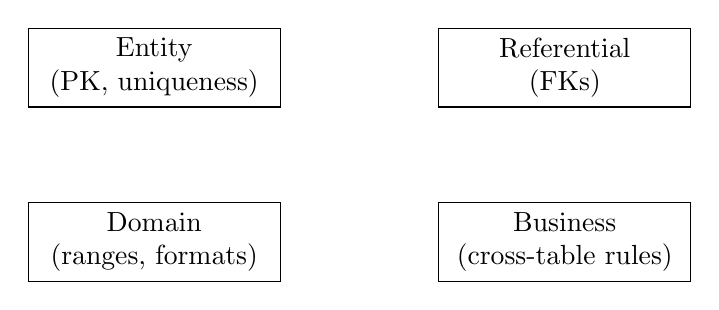
\begin{tikzpicture}[node distance=10mm]
  \node[draw, rectangle, minimum width=3.2cm, minimum height=1cm, align=center] (entity) {Entity\\(PK, uniqueness)};
  \node[draw, rectangle, minimum width=3.2cm, minimum height=1cm, align=center, right=20mm of entity] (ref) {Referential\\(FKs)};
  \node[draw, rectangle, minimum width=3.2cm, minimum height=1cm, align=center, below=12mm of entity] (domain) {Domain\\(ranges, formats)};
  \node[draw, rectangle, minimum width=3.2cm, minimum height=1cm, align=center, right=20mm of domain] (business) {Business\\(cross-table rules)};
\end{tikzpicture}
\end{document}
